\fontfamily{\sfdefault}\selectfont
% XCircuit output "pi_pz_plot.tex" for LaTeX input from pi_pz_plot.ps
\def\putbox#1#2#3#4{\makebox[0.00000in][l]{\makebox[#1][l]{}\raisebox{\baselineskip}[0.00000in][0.00000in]{\raisebox{#2}[0.00000in][0.00000in]{\scalebox{#3}{#4}}}}}
\def\rightbox#1{\makebox[0.00000in][r]{#1}}
\def\centbox#1{\makebox[0.00000in]{#1}}
\def\topbox#1{\raisebox{-0.60\baselineskip}[0.00000in][0.00000in]{#1}}
\def\midbox#1{\raisebox{-0.20\baselineskip}[0.00000in][0.00000in]{#1}}
   \scalebox{1}{
   \normalsize
   \parbox{4.20000in}{
   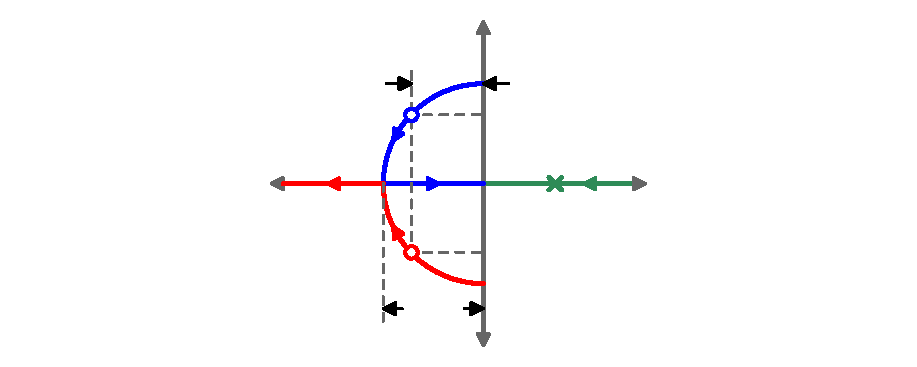
\includegraphics[scale=0.70000]{./figs/pi_pz_plot.pdf}\\
   % translate x=800 y=416 scale 0.38
   \putbox{2.85600in}{0.67900in}{1.20}{$\Re(s)$}%
   \putbox{2.30300in}{1.52600in}{1.20}{$\Im(s)$}%
   \putbox{1.89000in}{0.21700in}{1.20}{$\sqrt{\mathrm{K}}$}%
   \putbox{1.45600in}{1.36500in}{1.20}{$\zeta\sqrt{\mathrm{K}}$}%
   \putbox{2.38700in}{0.95900in}{1.20}{$\sqrt{\mathrm{K}}/2\zeta$}%
   } % close 'parbox'
   } % close 'scalebox'
   \vspace{-\baselineskip} % this is not necessary, but looks better
\fontfamily{\rmdefault}\selectfont
